\subsection{Counterfactual bias audit}
We scored 600 randomly chosen test pairs (69 postings) under 40 names and seven proxy cues
(Section~\ref{sec:audit}), once with the redaction front end and once with it disabled, each time using a
linear head trained under the same setting. Table~\ref{tab:audit} and Fig.~\ref{fig:audit} summarise the
result; the standard deviation of the score over these pairs is 14.8 points.

\emph{Explicit name cues.} With redaction on, the 40 names produce byte-identical redacted text, and the
score is identical to the last digit for every one of the 600 pairs. This is true by construction, and it
is what the first version of our audit failed to show: the audit had revealed that the header-name pattern
could span a newline and then be rejected by a section-header filter, leaving names in place for up to
1.46 points of variation. We fixed the pattern, added regression tests, and re-ran every experiment in this paper;
accuracy moved by at most 0.006 macro-F1. With redaction off, the name still has an effect on individual pairs
(up to 2.2 points) but not a systematic one: the largest gap between the ten cell means is 0.15 points, and
white-male versus black-male and versus black-female differences are not detectable (paired permutation
$p=0.50$ and $p=0.79$). The absence of a detectable name effect in \emph{this} model should not be taken as
evidence that name-sensitivity is absent in other systems. Our head weights relational features and sees names
only as rare tokens, whereas an embedding retriever that ranks by similarity of the whole document lets the name
enter the score directly, which is the setting in which large effects were reported \cite{wilson2024silicon}.

\emph{Proxy cues.} Redaction does not remove, and does not claim to remove, affinity organisations, hobbies or
career-break reasons. Each of these changes the score by a small but non-zero amount relative to a neutral line
of similar length: $-0.13$ points for a Black-affinity organisation, $-0.22$ for an East-Asian-affinity one,
$-0.11$ for female-coded versus $-0.05$ for male-coded hobbies (difference $p<0.001$) and $-0.10$ for a
childcare career break. About 1\% of decisions flip. These effects are tiny compared with the score's
spread (below 0.02 standard deviations), but they are measurable, are identical with and without redaction,
and point in the direction that audit studies of human and machine screeners would lead one to worry about.
The row ``named gendered org'' needs care. With redaction on, the cue is replaced by a placeholder, which differs
from the control line, so $-0.47$ measures the placeholder and not gender; with redaction off the same cue
moves the score by $-0.09$. A cleaner control that passes through the same redactor is a straightforward fix we
have not yet run.

\begin{table}[t]
\caption{Counterfactual audit of M3 on 600 test pairs. $\Delta$ score is in points of the 0--100 fit score
relative to a neutral control line; flips is the share of pairs whose decision band changes.}
\label{tab:audit}
\centering\scriptsize
\resizebox{\columnwidth}{!}{\begin{tabular}{l rr rr}
\toprule
 & \multicolumn{2}{c}{Redaction on} & \multicolumn{2}{c}{Redaction off} \\
\cmidrule(lr){2-3}\cmidrule(lr){4-5}
Cue vs. control line & $\Delta$ score [95\% CI] & flips & $\Delta$ score [95\% CI] & flips \\
\midrule
affinity org: black & $-$0.13 [$-$0.19, $-$0.08] & 1.2\% & $-$0.13 [$-$0.19, $-$0.07] & 1.3\% \\
affinity org: hispanic & $-$0.03 [$-$0.09, +0.03] & 1.3\% & $-$0.04 [$-$0.10, +0.02] & 1.0\% \\
affinity org: east asian & $-$0.22 [$-$0.33, $-$0.14] & 1.3\% & $-$0.22 [$-$0.32, $-$0.13] & 1.2\% \\
hobbies: female coded & $-$0.11 [$-$0.20, $-$0.03] & 1.2\% & $-$0.12 [$-$0.20, $-$0.03] & 0.8\% \\
hobbies: male coded & $-$0.05 [$-$0.11, +0.00] & 1.0\% & $-$0.05 [$-$0.12, $-$0.00] & 1.0\% \\
career break: childcare & $-$0.10 [$-$0.17, $-$0.05] & 1.0\% & $-$0.10 [$-$0.17, $-$0.05] & 1.0\% \\
named gendered org: female & $-$0.47 [$-$0.63, $-$0.32] & 2.2\% & $-$0.09 [$-$0.18, $-$0.01] & 1.3\% \\
\midrule
largest gap between name-cell means & \multicolumn{2}{c}{0.000} & \multicolumn{2}{c}{0.154} \\
largest per-pair change across 40 names & \multicolumn{2}{c}{0.000} & \multicolumn{2}{c}{2.205} \\
\bottomrule
\end{tabular}}
\end{table}

\begin{figure}[t]
\centering
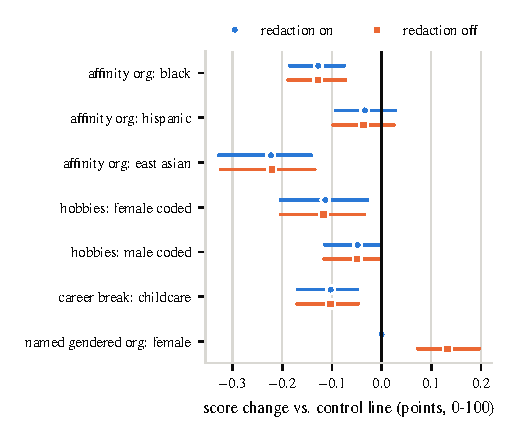
\includegraphics[width=\columnwidth]{figures/fig_audit.pdf}
\caption{Score change for each proxy cue relative to its control line, with and without redaction
(95\% intervals, bootstrap over postings).}
\label{fig:audit}
\end{figure}
